\chapter{Kapitola 2}
Lorem ipsum dolor sit amet, consectetur adipiscing elit.
Aliquam nunc magna, sollicitudin id leo eu, viverra congue risus.
Aliquam consequat ipsum ut erat placerat consequat nec at diam. 
Aenean est odio, molestie sit amet nunc in, pretium luctus elit. 
Donec imperdiet orci vel porttitor placerat. 
Proin ut hendrerit elit, ultricies accumsan urna. 
Vivamus condimentum lorem viverra lectus finibus, nec volutpat turpis auctor.
Cras quis felis non lorem consectetur interdum eu eu sem. 
Proin sit amet feugiat metus. 
Ut vitae orci a enim vestibulum porta:
\begin{itemize} % odrážkový seznam
    \item lorem
    \item ipsum
    \item lorem ipsum
    \item lipsum
\end{itemize}

\begin{table}[h]
    \centering
    \resizebox{\textwidth}{!}{%
    \begin{tabular}{@{}l|lll@{}}
        & \textbf{Průmyslová řešení} & \textbf{„Kutilská“ řešení} & \textbf{PROTOPlant}                                                                                   \\ \midrule
    \textbf{Dodání}      & Výroba na zakázku          & „Vyrob si sám“             & \begin{tabular}[c]{@{}l@{}}Možnost sestavení přímo doma, \\ nebo dodání \B{hotového} systému\end{tabular} \\
    \textbf{Cena}        & Drahá ($>$~10~000~Kč)      & Levná ($<$~10~000~Kč)      & Kompromis cena -- výkon (již od 2~500~Kč)                                                                               \\
    \textbf{Ovládání}    & Komplexní                  & Jednoduché (většinou)      & Jednoduché                                                                                            \\
    \textbf{Konektivita} & Většinou ethernet          & Často Wi-Fi                & \begin{tabular}[c]{@{}l@{}}Wi-Fi, Bluetooth, \\ možnost přidání podpory Ethernetu\end{tabular}        \\
    \textbf{Řízení}      & PLC                        & Většinou Arduino           & ESP32                                                                                                 \\ \bottomrule
    \textbf{Modularita}  & Ano                        & Ne                         & Ano                                                                                                   \\
    \textbf{Univerzálnost}& Ano                       & Ne                         & Ano                                                                                                   \\ 
    \textbf{Open-source} & Ne                         & Většinou ano               & Ano                                                                                                   \\ \bottomrule    
    \end{tabular}%
    }
    \caption{Tabulka srovnání PROTOPlantu a~jiných řešení.}
    \label{tab:COMPARATION}
\end{table}

\begin{figure}[htbp]
    \centering
    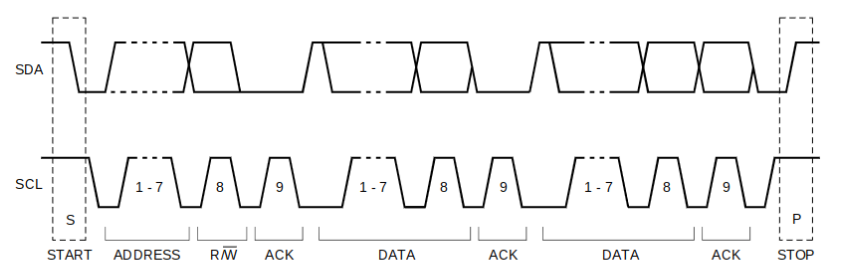
\includegraphics[width=\textwidth]{img/I2C.png}
    \caption{Celý datový přenos po I2C sběrnici. Převzato z~\cite{I2C_specs}}
    \label{fig:I2C-protocol}
 \end{figure}
 
\noindent\B{Lipsum} -- lorem ipsum dolor sit amet, consectetur adipiscing elit.
Aliquam nunc magna, sollicitudin id leo eu, viverra congue risus.
Aliquam consequat ipsum ut erat placerat consequat nec at diam. 
Aenean est odio, molestie sit amet nunc in, pretium luctus elit. 
Donec imperdiet orci vel porttitor placerat. 
Proin ut hendrerit elit, ultricies accumsan urna. 
Vivamus condimentum lorem viverra lectus finibus, nec volutpat turpis auctor.
Cras quis felis non lorem consectetur interdum eu eu sem. 
Proin sit amet feugiat metus. 
Ut vitae orci a enim vestibulum porta. \newline

\section{Sumarizace}
Nabídka řešení v~tomto oboru je velmi chudá.
Na jedné straně stojí průmyslová řešení, která jsou drahá a~dodávají se primárně do skleníků velkých zemědělských firem.
Na opačném břehu jsou řešení amatérská. 
Ta jsou ovšem buďto naprosto nepoužitelná v~běžně velkém skleníku (primárně je uživatelé vyrábí pro malá pařeniště), nebo neuniverzální.

\newpage